\chapter*{Preface}%
\pdfbookmark{Preface}{preface}%
%
After writing \inQuotes{\citetitle{W2009GOATAA}}~\cite{W2009GOATAA} as PhD student a long time ago, I now want to write a more \emph{practical} guide to optimization and metaheuristics.
Currently, this book is in an early stage of development and work-in-progress, so expect many changes.

This book tries to introduce optimization in an accessible way for an audience of undergraduate and graduate students without background in the field.
It tries to provide an intuition about how optimization algorithms work in practice, how to recognize optimization problems and the basic structure behind them, what things to look for when solving an optimization problem, and how to get from a simple, working, \inQuotes{proof-of-concept} approach to an efficient algorithm for a given problem.

We follow a \inQuotes{learning-by-doing} approach by trying to solve one practical optimization problem as example theme throughout the book.
All algorithms are directly implemented and applied to that problem after we introduce them.
This allows us to discuss their strengths and weaknesses based on actual results.
We learn how to compare the performance of different algorithms.
We try to improve the algorithms step-by-step, moving from very simple approaches, which do not work well, to efficient metaheuristics.

We use concrete examples and algorithm implementations written in \python~\cite{programmingWithPython}.
The source code is freely as part of the \moptipy\ package under the GNU GENERAL PUBLIC LICENSE Version~3, 29~June~2007.
The code listings in the book will usually be abridged excerpts.

In order to fully understand the code examples, we recommend the reader to familiarize themselves with  \python, \numpy, and \matplotlib.
Of course, if you just read this book to learn about algorithms, you can ignore the source code examples.

This book is released under the \emph{Attribution-NonCommercial-ShareAlike~4.0 International license} (\href{http://creativecommons.org/licenses/by-nc-sa/4.0/}{\mbox{CC~BY-NC-SA~4.0}}).
You can freely share it.
Please do not print it, though, to preserve the environment.
%
\strut\vfill\strut%
%
\copyrightBlock{2024--2026}%
%
\clearpage%
%
\strut\vfill\strut%
%
\begin{center}%
\noindent\resizebox{\linewidth}{!}{%
\begin{tabular}{c@{~~~~~~~~}c}%
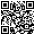
\includegraphics[width=7cm]{\currentDir/bookUrl}&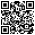
\includegraphics[width=7cm]{\currentDir/courseUrl}\\\relax%
{\huge{[\expandafter\href{\oaUrl/oa.pdf}{book pdf}]}}&{\huge{[\expandafter\href{\oaUrl}{course website}]}}\\%
\end{tabular}}%
\\[12pt]\noindent%
\resizebox{0.85\linewidth}{!}{\expandafter\url{\oaUrl}}%
\end{center}%
%
\strut\vfill\strut%
This book was built using the following software:%
\gitExec{exec:versions}{}{}{text/front/preface/dependencyVersions.sh}%
\lstinputlisting[style=text_style]{\gitFile{exec:versions}}%
